\documentclass[12pt]{article}

\usepackage[top=1in, bottom=1in, left=1in, right=1in]{geometry}
\usepackage{authblk}
\usepackage[utf8]{inputenc}
\usepackage{siunitx}
\usepackage{graphicx}
\usepackage{subcaption}
\usepackage{float}
\usepackage{enumitem}
\usepackage[dvipsnames]{xcolor}
\usepackage{caption}
\usepackage{amssymb}

\usepackage{xspace,graphicx,amsmath,amsthm,amssymb,xcolor}

\usepackage{varwidth}
\newcommand{\fcodebox}[1]{%
    \framebox{\codebox{#1}}%
}
\newcommand{\codebox}[1]{%
        \begin{varwidth}{\linewidth}%
        \begin{tabbing}%
            ~~~\=\quad\=\quad\=\quad\=\quad\=\quad\=\kill
            #1
        \end{tabbing}%
        \end{varwidth}%
}









\title{CS 517: A tool for Job Shop Problem \\ Final Report}

\date{Spring 2019}
\author{Wei-Jen Chen, Weijie Mo}

\makeatletter
\let\inserttitle\@title
\let\insertdate\@date

\begin{document}

\begin{center}
  \LARGE{\inserttitle}

  \Large{\@author}
\end{center}

\hrulefill

\section*{Abstract}
Job Shop Scheduling problem is a complicated scheduling problem.  In JSS problem, there are many different tasks which can be processed by many different machine at many different time. In this document, we will show the reduction to 3-SAT problem and create a tool to solve this problem by z3 sat-solver. We will evaluate the tool by comparing the behavior between our tool and Google OR tool. 
\section*{Preface}
At first we are planning to do the research in the topic that not many people did before. Therefore we choose to do research in Kirkman's schoolgirl problem. Kirkman's schoolgirl problem(1850s) is a combinatorial optimisation scheduling problem, and it can be transformed to another well-known social golfer problem(1998). However, in “An Improved SAT Formulation for the Social Golfer Problem”[1], we learn that this problem is NP-complete only if when deciding whether a partially filled schedule can be completed to conflict-free one, and the computational complexity of this problem is currently unknown. Therefore, we plan to do another scheduling problem we found in Google OR-Tools project, which is Job Shop Scheduling problem(JSS)[2]. At the meantime, we found a very detailed tutorial for z3 SAT-solver written by two Microsoft employee[3]. Therefore, our new plan is that we will build a tool to solve JSS by using z3 SAT solver in python, and we can compare our tool to Google OR-Tool in evaluation section if necessary. 
\section*{Background}
JSS is an optimization problem in CS and operation research, and it can be extended to many different problem depend on the given “constraints”. In this document, we will follow the Google Project’s version[2]: Suppose there are many jobs which are processed by several machines, Job shop scheduling problem is to minimize the length of the schedule under the following constraints:

\begin{enumerate}
 \item Each job consists of a sequence of tasks, which must be performed in a given order

  \item Each task must be processed on a specific(correspond) machine

   \item No task can be started until the previous task is completed

    \item A machine can only work on one task at one time

     \item Once a machine start a task, it need to run to complete


\end{enumerate}
Here is the example from Google’s project: Each task below is labeled by a pair of numbers (m, p) where m is the number of the machine the task must be processed on and p is the processing time of the task — the amount of time it requires. (The numbering of jobs and machines starts at 0.)
\begin{itemize}
\item job 0 = [(0, 3), (1, 2), (2, 2)]
\item job 1 = [(0, 2), (2, 1), (1, 4)]
\item job 2 = [(1, 4), (2, 3)]
\end{itemize}

\begin{figure}[H]
\centering
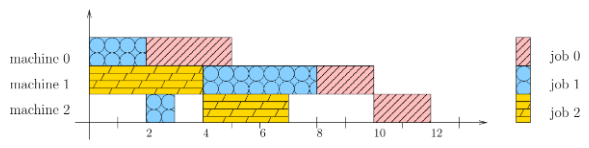
\includegraphics[width=4in]{img/1.PNG}
\caption{one possible solution for Google JSS example}
\end{figure}
\section*{Reduction}
First, we define some variable for JSS problem. We have start ($S${\scriptsize$i,j$}) for the start time of $j$-th task for job $i$.  Each task start at $S${\scriptsize$i,j$} and run $T${\scriptsize$i,j$} units of time, where $T${\scriptsize$i,j$} denotes the duration of $j$-th task of job $i$. In classic JSS problem, there are only 2 constraints:

\begin{enumerate}
 \item Precedence \\
A precedence constraint between two consecutive tasks $T${\scriptsize$i,j$} and $T${\scriptsize$i,j+1$} is encoded using
the inequality $S${\scriptsize$i,j+1$} $\geq$ $S${\scriptsize$i,j$} + $S${\scriptsize$i,j$}. This inequality states that the start-time of task $j+1$ must be greater than or equal to the start-time of task $j$ plus its duration.


\item Resource Capacity \\
 A resource constraint between two tasks from different jobs $i$ and $i$' requiring the same machine $j$ is encoded using the formula \\
 ($S${\scriptsize$i,j$} $\geq$ $S${\scriptsize$i$',$j$} + $T${\scriptsize$i$',$j$}) $\vee$ ($S${\scriptsize$i$',$j$} $\geq$ $S${\scriptsize$i,j$} + $T${\scriptsize$i,j$}) , which states that the two tasks do not overlap. 


\end{enumerate}
Moreover, other than the 2 main constraints above, we need some other constraint in programming.

\begin{enumerate}
\setcounter{enumi}{2}
 \item  Start-time for the first task of each job need to be greater or equal to zero,
 that is\\ $S${\scriptsize$i$,0} $\geq$ 0



\item At the end, we define a variable $max$(makespan). And we want to decide if there is a schedule such that end-time of the last task is less or equal max time, that is $S${\scriptsize$i,n$} + $T${\scriptsize$i,n$} $\leq$ $max$(makespan), where $n$ is the index number of last task for each job.




\end{enumerate}
We conclude the constraints in arbitrary sentence in the following table. 

\begin{figure}[H]
\centering
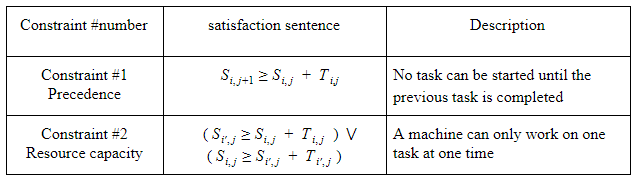
\includegraphics[width=6in]{img/2.PNG}

\end{figure}
We will continue using the example from Google project to generate the SMT formula:

\begin{figure}[H]
\centering
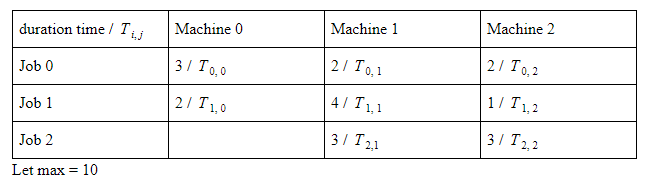
\includegraphics[width=6in]{img/3.PNG}

\end{figure}

\subsection*{Encoding:}
($S${\scriptsize0,0} $\geq$ 0) $\wedge$ ($S${\scriptsize0,1} $\geq$ $S${\scriptsize0,0} + 3) $\wedge$ ($S${\scriptsize0,2} $\geq$ $S${\scriptsize0,1} + 2) $\wedge$ ($S${\scriptsize0,2} + 2 $\leq$ 10) $\wedge$ \\
($S${\scriptsize1,0} $\geq$ 0) $\wedge$ ($S${\scriptsize1,1} $\geq$ $S${\scriptsize1,0} + 2) $\wedge$ ($S${\scriptsize1,2} $\geq$ $S${\scriptsize1,1} + 4) $\wedge$ ($S${\scriptsize1,2} + 1 $\leq$ 10) $\wedge$ \\
($S${\scriptsize2,1} $\geq$ 0) $\wedge$ ($S${\scriptsize2,2} $\geq$ $S${\scriptsize2,1} + 3)  $\wedge$ ($S${\scriptsize2,2} + 3 $\leq$ 10) $\wedge$ \\
(($S${\scriptsize0,0} $\geq$ $S${\scriptsize1,0} + 2) $\vee$ ($S${\scriptsize1,0} $\geq$ $S${\scriptsize0,0} + 3)) $\wedge$ \\
(($S${\scriptsize0,1} $\geq$ $S${\scriptsize1,1} + 4) $\vee$ ($S${\scriptsize1,1} $\geq$ $S${\scriptsize0,1} + 2)) $\wedge$ \\
(($S${\scriptsize0,1} $\geq$ $S${\scriptsize2,1} + 3) $\vee$ ($S${\scriptsize2,1} $\geq$ $S${\scriptsize0,1} + 2)) $\wedge$ \\
(($S${\scriptsize1,1} $\geq$ $S${\scriptsize2,1} + 3) $\vee$ ($S${\scriptsize2,1} $\geq$ $S${\scriptsize1,1} + 4)) $\wedge$ \\
(($S${\scriptsize0,2} $\geq$ $S${\scriptsize1,2} + 1) $\vee$ ($S${\scriptsize1,2} $\geq$ $S${\scriptsize0,2} + 2)) $\wedge$ \\
(($S${\scriptsize0,2} $\geq$ $S${\scriptsize2,2} + 3) $\vee$ ($S${\scriptsize2,2} $\geq$ $S${\scriptsize0,2} + 2)) $\wedge$ \\
(($S${\scriptsize1,2} $\geq$ $S${\scriptsize2,2} + 3) $\vee$ ($S${\scriptsize2,2} $\geq$ $S${\scriptsize1,2} + 1)) 
\newpage
\section*{Code}

We will show our partial code in the following table. For completed code, please check our github at the end of this chapter. \\

\fcodebox{


\#  items can not overlap: \\
def no\_items\_overlap (s, lst): \\
\>\>for pair in itertools.combinations(lst, r = 2): \\
\>\>\>\>no\_interval\_overlap(s, (pair[0][1], pair[0][2]), (pair[1][1], pair[1][2])) \\

\#  intervals can not overlap: \\
def no\_interval\_overlap (s, i1, i2): \\
\>\>(i1\_begin, i1\_end) = i1 \\
\>\>(i2\_begin, i2\_end) = i2 \\
\>\>s.add(Or(i1\_begin $\geq$ i2\_end, i1\_end <= i2\_begin)) \\
    
for job in range(len(jobs)): \\
\>\>former\_task\_end = None \\
\>\>jobs\_list\_tmp = [] \\
 
\>\>for t in jobs[job]: \\
\>\>\>\>machine = t[0] \\
\>\>\>\>time\_used = t[1] \\
\#set  variables: \\
\>\>begin = Int('j\_\%d\_task\_\%d\_\%d\_begin' \% (job, machine, time\_used)) \\
\>\>end = Int('j\_\%d\_task\_\%d\_\%d\_end' \% (job, machine, time\_used))\\
        
\#check whether it is avaliable to add tasks\\
\>\>if (begin,end) not in tasks\_machines[machine]:\\
\>\>\>\>tasks\_machines[machine].append((job,begin,end))\\

\#check whether it is avaliable to add jobs        \\
\>\>if (begin,end) not in jobs\_list\_tmp:\\
\>\>\>\>jobs\_list\_tmp.append((job,begin,end)) \\

\# task start from time $\geq$ 0\\
\>\>sol.add(begin $\geq$ 0)\\

\# no task end after makespan:\\
\>\>sol.add(end $\leq$ makespan)\\
         
        

\# end time is fixed with begin time:\\
\>\>sol.add(end == begin+time\_used)\\


\# no task begin before the last task end:\\
\>\>if former\_task\_end != None:\\
\>\>\>\>sol.add(begin $\geq$ former\_task\_end)\\
\>\>\>\>former\_task\_end = end\\
\>\>\>\>jobs\_list.append(jobs\_list\_tmp)\\

}
\newpage
\fcodebox{
\# no tasks overlap on machines:\\
for tasks\_for\_machine in tasks\_machines:\\
\>\>no\_items\_overlap(sol, tasks\_for\_machine)\\

\# no tasks overlap on each jobs:\\
for jobs\_list\_tmp in jobs\_list:\\
\>\>no\_items\_overlap(sol, jobs\_list\_tmp)\\


\>\>min = sol.minimize(makespan)\\

\#unknown = CheckSatResult(Z3\_L\_UNDEF)\\


if sol.check() == unknown:\\
\>\>print ("the result is unknown")\\
\>\>exit(0)\\

\#sat = CheckSatResult(Z3\_L\_TRUE)\\
\#unsat = CheckSatResult(Z3\_L\_FALSE)\\
elif sol.check() == unsat:\\
\>\>print ("the result is unsat")\\
\>\>exit(0)\\

\#sol.lower is to check&ensure result returned by maximize/minimize \\
\>\>sol.lower(min)\\

\#m\_sol is to return optimized machine using schedule\\
\>\>m\_sol = sol.model()\\


    
    }

Github: https://github.com/javamore/SAT-jobshop/blob/master/jobshop.py
\section*{Evaluation}
We have done several sets of tests by using different size of data($machine$ x $job$), and we let the number of tasks equal to the number of jobs(tasks can be less than jobs). We use the data set retrieved from SAS web site[6], one of the test result is shown as follow:\\
\subsection*{Test result: 10x10}
Machine Number: 10,  Job Number: 10
\begin{itemize}
 
\item Job0: [(2,44),(3,5),(5,58),(4,97),(0,9),(7,84),(8,77),(9,96),(1,58),(6,89)],  

\item Job1: [(4,15),(7,1),(1,87),(8,57),(0,77),(3,85),(2,81),(5,39),(9,73),(6,21)],  

\item job2: [(9,82),(6,22),(4,10),(3,70),(1,49),(0,40),(8,34),(2,48),(7,80),(5,71)], 

\item job3: [(1,91),(2,17),(7,62),(5,75),(8,47),(4,11),(3,7),(6,72),(9,35),(0,55)], 

\item job4: [(6,71),(1,90),(3,75),(0,64),(2,94),(8,15),(4,12),(7,67),(9,20),(5,50)], 

\item job5: [(7,70),(5,93),(8,77),(2,29),(4,58),(6,93),(3,68),(1,57),(9,7),(0,52)],   

\item job6: [(6,87),(1,63),(4,26),(5,6),(2,82),(3,27),(7,56),(8,48),(9,36),(0,95)], 

\item job7: [(0,36),(5,15),(8,41),(9,78),(3,76),(6,84),(4,30),(7,76),(2,36),(1,8)], 

\item job8: [(5,88),(2,81),(3,13),(6,82),(4,54),(7,13),(8,29),(9,40),(1,78),(0,75)], 

\item job9: [(9,88),(4,54),(6,64),(7,32),(0,52),(2,6),(8,54),(5,82),(3,6),(1,26)]   

\end{itemize}

\begin{figure}[H]
\centering
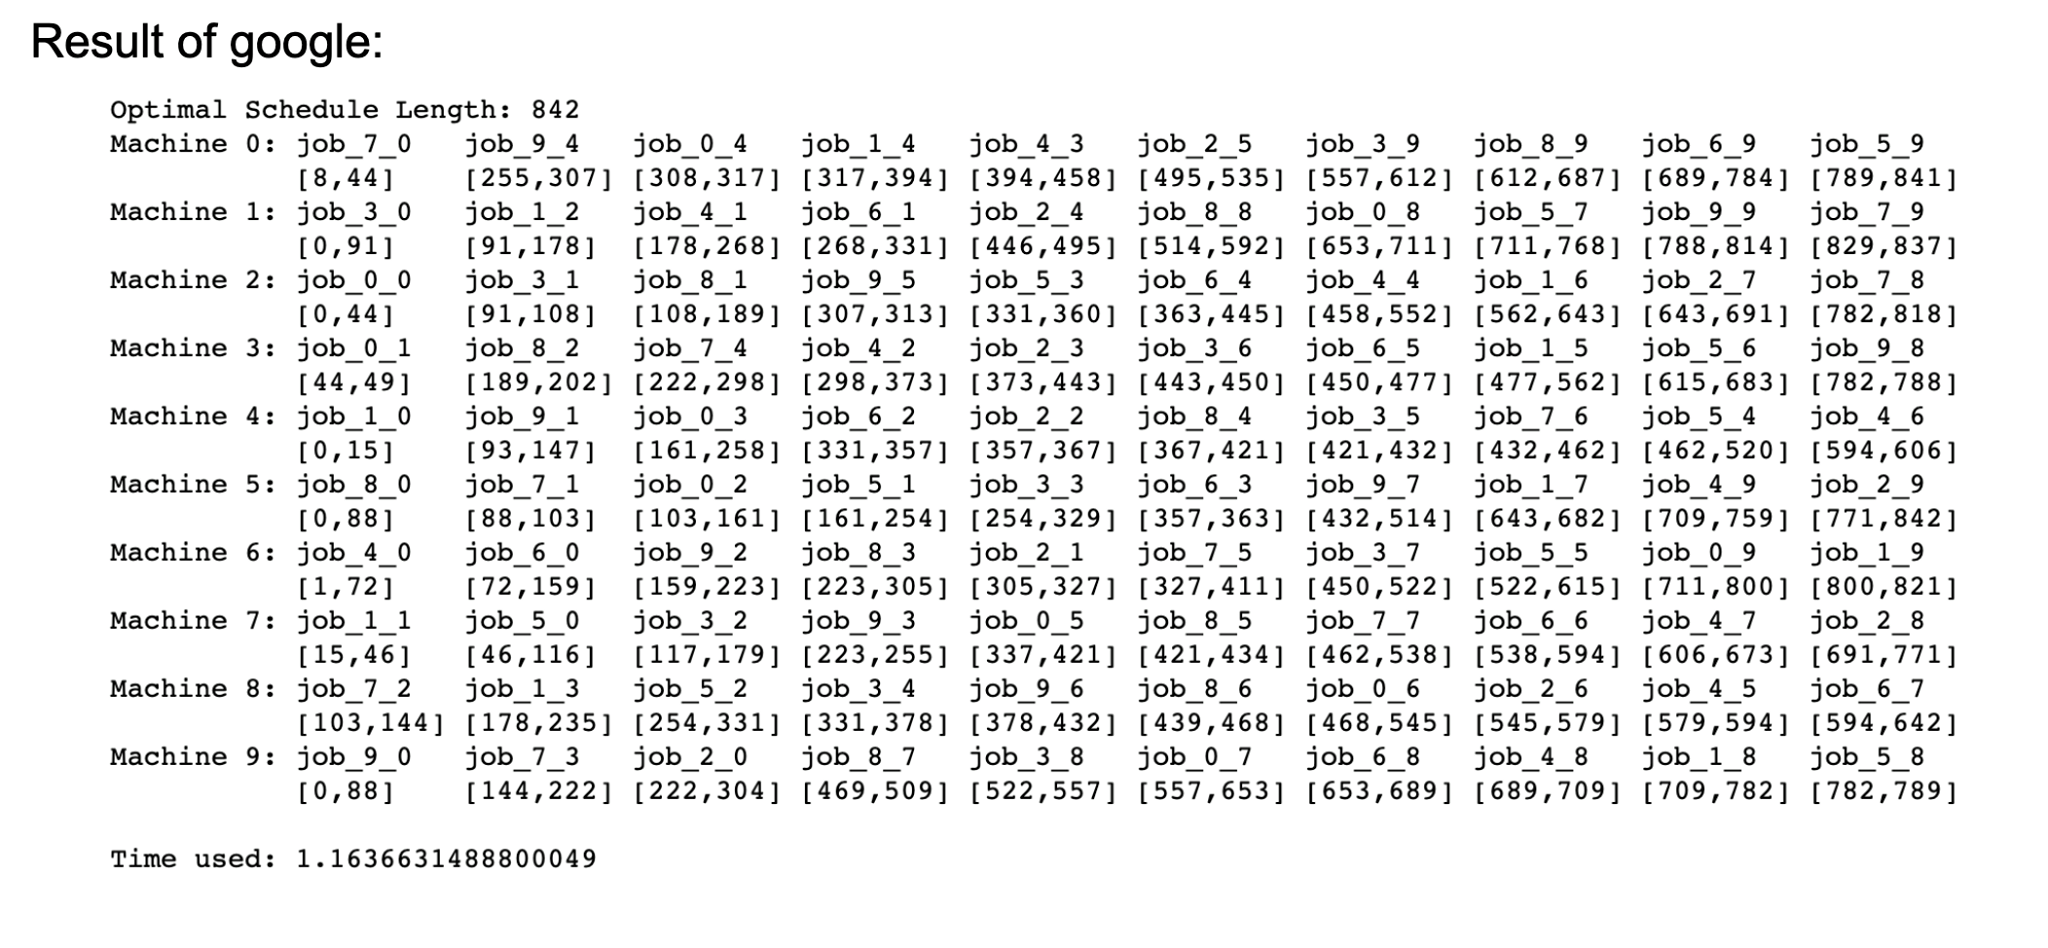
\includegraphics[width=4in]{img/google.png}
\caption{10x10 testing result of Google-OR-tool}
\end{figure}

\begin{figure}[H]
\centering
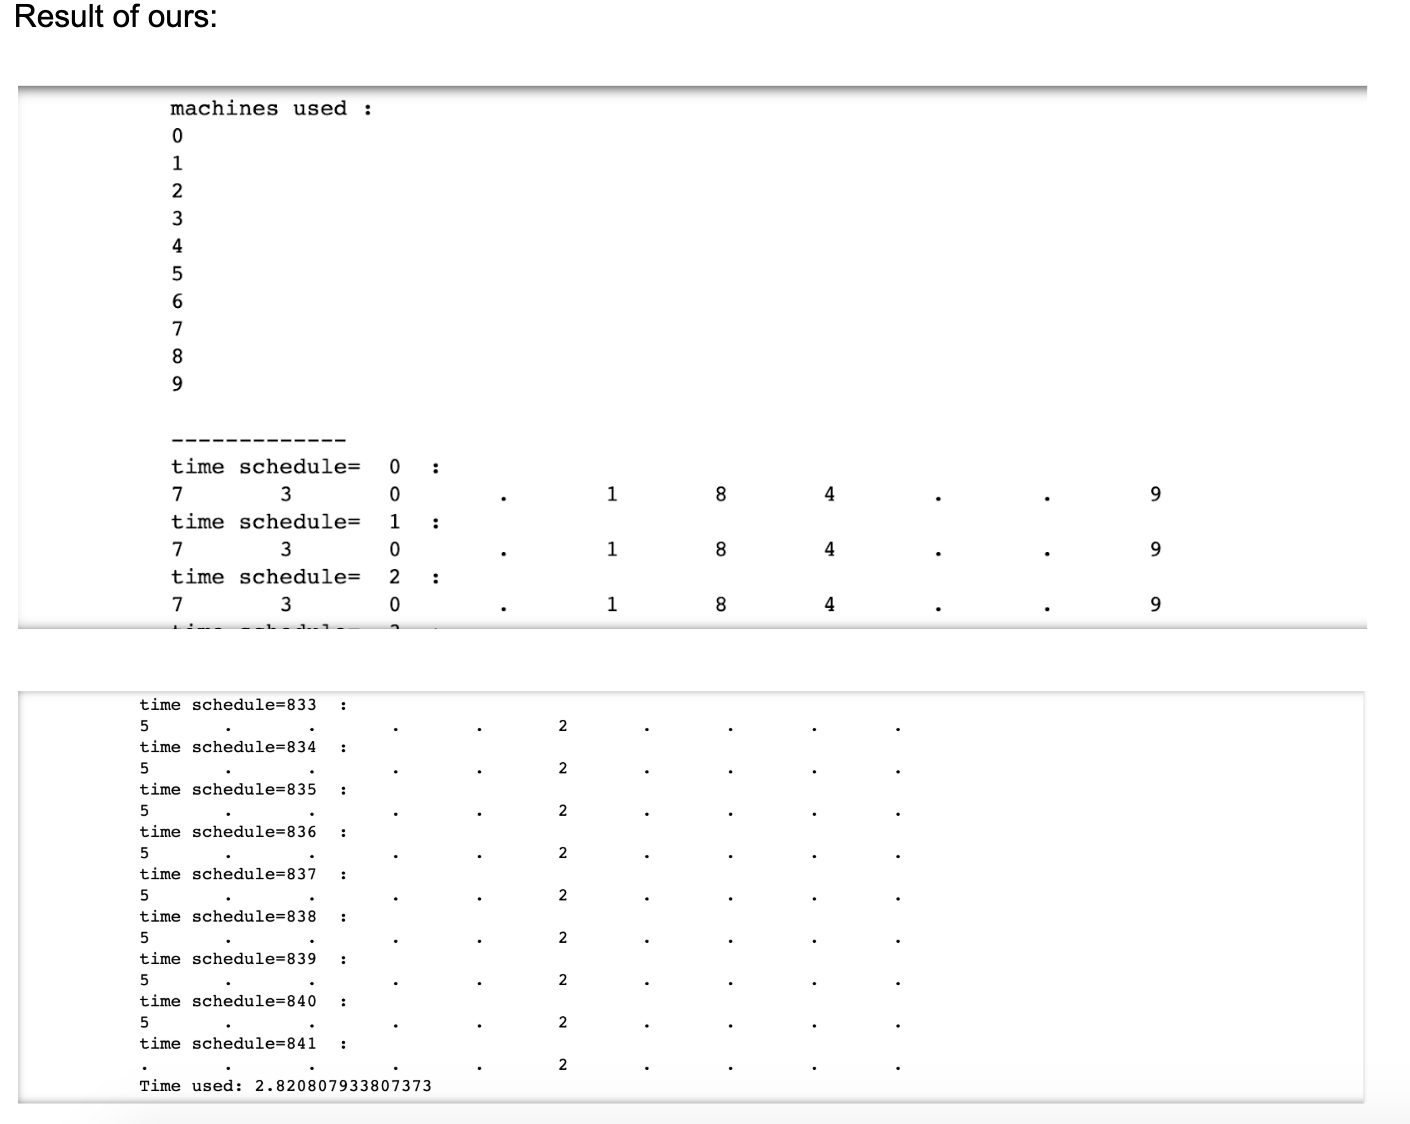
\includegraphics[width=4in]{img/sat.png}
\caption{10x10 testing result of our Z3-tool}
\end{figure}


By testing the data set 6x6, 8x8, 10x10, we learn that our Z3-tool can generate same
answer as Google-OR-tool.(\*Note that our schedule length start with 0 while
Google-OR-tool start with 1, therefore our result will be 1 unit time less than
google's) However, our performance is not as good as Google's. While the data set
comes to 15x15, our tool seems will run forever(more than 15 minutes) while Google's
only run 41.51(sec). When the data set comes to 20x20, our tool will run more than 15 minutes, while Google's only run 93.17(sec).      

\begin{figure}[H]
\centering
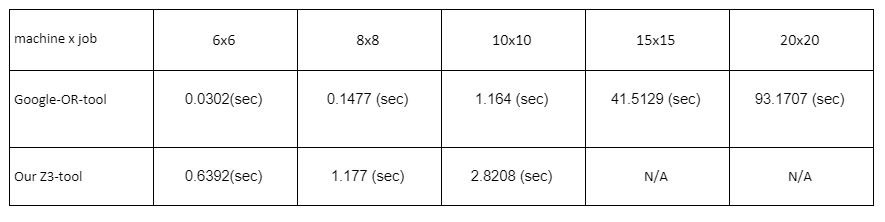
\includegraphics[width=6in]{img/4.PNG}
\caption{Result Table}
\end{figure}
\section*{Conclusion}
During our research in JSS problem, we learned that there are some other new technics come out recently. For example, in 2004, Reduced Sat Formula (RSF)[4] was published. RSF is a new codification of JSS problem that need fewer clauses in the SAT formula for JSS problem instances than our work. Moreover, this same group come out a more efficient algorithm, which is RandTaunt [5]. However, because we change the topic 2 weeks ago before the deadline, we don’t have much time to get familiar with those new idea. Therefore, we use relatively old algorithm to build our tool. In the future, we will try to implement those new ideas to our tool, and make our tool more efficient. 
\begin{thebibliography}{1}

\bibitem{} Markus Triska, Nysret Musliu. February 2010. {\em An Improved SAT Formulation for the Social Golfer Problem.} Springer Science+Business Media, LLC 2010

\bibitem{}  Google-OR-Tool. {\em The Job Shop Problem}. Goole Developer

\bibitem{} Leonardo de Moura, Nikolaj Bjørner. {\em Z3 - a Tutorial}. Microsoft Research

\bibitem{} Solís, Juan Frausto and Marco Antonio Cruz-Chávez. {\em A Reduced Codification for the Logical Representation of Job Shop Scheduling Problems}. ICCSA (2004).

\bibitem{} Frausto-Solís, Juan et al. {\em A Very Efficient Algorithm to Representing Job Shop Scheduling as Satisfiability Problem. (2008). An Improved SAT Formulation for the Social Golfer Problem.
}

\bibitem{} SAS website. {\em SAS/OR(R)9.3 User's Guide: Constraint Programming} \\
http://support.sas.com/documentation/cdl/en/orcpug/63973/HTML/default/viewer.htm\#orc
pug\_clp\_sect048.htm

\end{thebibliography}


\end{document}